\documentclass[11pt]{article}
\usepackage{amsmath}
\usepackage{amssymb}
\usepackage{graphicx}
\usepackage{fancyhdr}
\usepackage{url}
\usepackage{enumerate}
\usepackage{titlesec}
\usepackage[colorlinks=true,urlcolor=blue]{hyperref}

\titlespacing{\subsubsection}{0pt}{0pt}{0pt}

% No page numbers
%\pagenumbering{gobble}

% INFORMATION SHEET (DO NOT EDIT THIS PART) ---------------------------------------------
\newcommand{\addinformationsheet}{
\clearpage
\thispagestyle{empty}
\begin{center}
\LARGE{\bf \textsf{Information sheet\\CS246: Mining Massive Data Sets}} \\*[4ex]
\end{center}
\vfill
\textbf{Assignment Submission } Fill in and include this information sheet with each of your assignments.  This page should be the last page of your submission.  Assignments are due at 11:59pm and are always due on a Thursday.  All students (SCPD and non-SCPD) must submit their homework via Gradescope (\url{http://www.gradescope.com}). Students can typeset or scan their homework. Make sure that you answer each (sub-)question on a separate page. That is, one answer per page regardless of the answer length. Students also need to upload their code on Gradescope. Put all the code for a single question into a single file and upload it.  
\\
\\
\textbf{Late Homework Policy } Each student will have a total of {\em two} late periods. {\em Homework are due on Thursdays at 11:59pm PT and one late period expires on the following Monday at 11:59pm PT}.  Only one late period may be used for an assignment.  Any homework received after 11:59pm PT on the Monday following the homework due date will receive no credit.  Once these late periods are exhausted, any assignments turned in late will receive no credit.
\\
\\
\textbf{Honor Code } We strongly encourage students to form study groups. Students may discuss and work on homework problems in groups. However, each student must write down their solutions independently, i.e., each student must understand the solution well enough in order to reconstruct it by him/herself.  Students should clearly mention the names of all the other students who were part of their discussion group. Using code or solutions obtained from the web (GitHub/Google/previous year's solutions etc.) is considered an honor code violation. We check all the submissions for plagiarism. We take the honor code very seriously and expect students to do the same. 
\vfill
}

% MARGINS (DO NOT EDIT) ---------------------------------------------
\oddsidemargin  0.25in \evensidemargin 0.25in \topmargin -0.5in
\headheight 0in \headsep 0.1in
\textwidth  6.5in \textheight 9in
\parskip 1.25ex  \parindent 0ex \footskip 20pt
% ---------------------------------------------------------------------------------

% HEADER (DO NOT EDIT) -----------------------------------------------
\newcommand{\problemnumber}{0}
\newcommand{\myname}{name}
\newfont{\myfont}{cmssbx10 scaled 1000}
\pagestyle{fancy}
\fancyhead{}
\fancyhead[L]{\myfont Question \problemnumber, Homework 2, CS246}
%\fancyhead[R]{\bssnine \myname}
\newcommand{\newquestion}[1]{
\clearpage % page break and flush floats
\renewcommand{\problemnumber}{#1} % set problem number for header
\phantom{}  % Put something on the page so it shows
}
% ---------------------------------------------------------------------------------


% BEGIN HOMEWORK HERE
\begin{document}

% Question 1(a)
\newquestion{1(a)}

Matrix $A$ is symmetric if $A^T = A$. We calculate
\begin{align*}
    (M M^T)^T &= (M^T)^T M^T = M M^T \text{,} \\
    (M^T M)^T &= M^T (M^T)^T = M^T M \text{,}
\end{align*}
where we used the rules $(A B)^T = B^T A^T$ and $(A^T)^T = A$.
We can see that both matrix products $M M^T$ and $M^T M$ are symmetric.

If the first matrix has dimensions $m \times n$, and is multiplied by a second matrix of dimensions $n \times p$, then the dimensions of the product matrix will be $m \times p$.
Say that matrix $M$ is of size $p \times q$, then matrix $M^T$ is of size $q \times p$. Therefore product of matrices $M M^T$ has dimensions $p \times p$ 
and the product of matrices $M^T M$ has dimensions $q \times p$. We conclude, that both are square matrices.

If all the values in a matrix $M$ are real, then also all the values in $M M^T$ and $M^T M$ are real, since every value is just a sum of products of real numbers.
Hence both $M M^T$ and $M^T M$ are real matrices.

If $M$ has complex values, then $M M^T$ and $M^T M$ are not always real. Here's an example
\[ M = 
\begin{bmatrix}
1 & i \\
2 & 1 \\
\end{bmatrix}
\]

\[ M M^T = 
\begin{bmatrix}
1 & i \\
2 & 1 \\
\end{bmatrix}
\begin{bmatrix}
1 & 2 \\
i & 1 \\
\end{bmatrix}
=
\begin{bmatrix}
0 & 2+i \\
2+i & 3 \\
\end{bmatrix}
\]


% Question 1(b)
\newquestion{1(b)}

$MM^T$ and $M^TM$ are square, symmetric, real matrices, therefore, they have eigenpairs. 
If $v$ is its eigenvector for eigenvalue $\lambda$ of matrix $M^TM$, then by definition, it holds 
that $$M^TM v = \lambda v\text{.}$$ Multiplying both sides from the left with $M$
gives $$MM^T(M v) = \lambda (Mv) \text{.}$$ Multiplication is possible since all dimensions are compatible.
We can see that $Mv$ is the eigenvector for eigenvalue $\lambda$ of matrix $MM^T$. From here it follows,
that $M^TM$ and $MM^T$ have the same eigenvalues.
% We can find its eigenvalues by 
% finding zeros of determinant $\det (A - \lambda I)$.
% We can easily see, that $\det (A^T - \lambda I) = \det (A - \lambda I)^T = \det (A - \lambda I)$,
% where first equality follows from rule that states $(A + B)^T = A^T + B^T$ and second equality follows from $\det A^T = \det A$
% for any two matrices $A$ and $B$ with compatible sizes.
% Therefore zeros of $\det (A^T - \lambda I)$ are exactly zeros of $\det (A - \lambda I)$. Hence square, real matrix $A$
% has the same eigenvalues as its transpose $A^T$.
% Since $M M^T$ and $M^T M$ are connected by transposition, they share same eigenvalues.

Eigenvectors of matrices $M M^T$ and $M^T M$ are not necesserly the same, as their sizes are not always the same.

% Question 1(c)
\newquestion{1(c)}

From part 1(a) we know that $M^T M$ is symmetric, square and real. From the decomposition described at the beginning 
of the question, we know that such a matrix can be written as $$M^T M = Q \Lambda Q^T \text{,}$$ where $\Lambda$ is diagonal matrix with
eigenvalues of $M^T M$ on its diagonal and $Q$ orthogonal matrix containing the eigenvectors of $M^T M$ as its columns.

% Question 1(d)
\newquestion{1(d)}

It is given that $M = U \Sigma V^T$. We can calculate transpose of $M$
$$M^T = (U \Sigma V^T)^T = (V^T)^T \Sigma^T U^T = V \Sigma^T U^T = V \Sigma U^T \text{,}$$ 
where in second equality we used $(A B)^T = B^T A^T$, in third we used $(A^T)^T = A$ and in the 
last one follows because for a diagonal matrix $\Sigma$ it holds $\Sigma = \Sigma^T$.

Knowing that $U$ is column-orthonormal, therefore $U^T U = I$, we can calculate the product
$$M^T M = (V \Sigma U^T) (U \Sigma V^T) = V \Sigma (U^T U) \Sigma V^T = V \Sigma^2 V^T \text{.}$$ 

% Question 1(e)
\newquestion{1(e)}

Singular Value Decomposition of the given matrix $M$ is 
\[ U = 
\begin{bmatrix}
    -0.27854301 &  0.5 \\
    -0.27854301 & -0.5 \\
    -0.64993368 &  0.5 \\
    -0.64993368 & -0.5 \\
\end{bmatrix} 
\text{,} \] 
\[ 
\Sigma = 
\begin{bmatrix}
    7.61577311 & 0 \\
    0 & 1.41421356
\end{bmatrix}
\text{,}\\
\] 
\[
V^T = 
\begin{bmatrix}
    -0.70710678 & -0.70710678 \\
    -0.70710678 &  0.70710678 \\
\end{bmatrix}
\text{.}
\]

We computed eigenvector decomposition and got an array of eigenvalues
$$ Evals = \left[ 58\text{, } 2 \right]$$
and a matrix of eigenvectors
\[ Evecs = 
\begin{bmatrix}
    0.70710678 & -0.70710678 \\
    0.70710678 &  0.70710678 \\
\end{bmatrix}
\]

From parts (c) and (d) we assume $$M^T M = V \Sigma^2 V^T = P D P^T \text{,}$$
where $D$ is a diagonal matrix with elements from Evals on its diagonal and $P = Evecs$.
Second equality can be rewritten as $$ \Sigma^2 = V^T P D P^T  V \text{.}$$
If we denote $Q = V^T P$, we get $\Sigma^2 = Q D Q^T$.

From this we can see connection between matrix $V$ and matrix $Evecs$. We compute 
\[ Q = V^T \cdot Evecs = 
\begin{bmatrix}
    -0.70710678 & -0.70710678 \\
    -0.70710678 &  0.70710678 \\
\end{bmatrix}
\begin{bmatrix}
    0.70710678 & -0.70710678 \\
    0.70710678 &  0.70710678 \\
\end{bmatrix}
= 
\begin{bmatrix}
    - 1 & 0 \\
    0 & 1 
\end{bmatrix}
\]
Therefore in our example $V$ is obtained by reflecting $Evecs$ across $x$-axis. In other words, we can compute $V$ as
\[ V = Q^{-1} \cdot Evecs \text{,}\] 
where $Q^{-1} = 
\begin{pmatrix}
    1 & 0 \\ 
    0 & -1 \\
\end{pmatrix}$ is reflection matrix across $x$-axis.

Now, we can observe the equation $\Sigma^2 = Q D Q^T$. Since $Q$ is diagonal with values $\pm 1$ and $\Sigma$ and $D$ are also diagonal,
every element in $D$ is a square of corresponding value in matrix $\Sigma$. In essence, we have the relationship $\Sigma^2 = D$. 
Recall that matrix $D$ contains eigenvalues along its diagonal, 
while matrix $\Sigma$ contains singular values along its diagonal. Consequently, this relationship indicates that every eigenvector corresponds to the square of a singular value.

% Question 2(a)
\newquestion{2(a)}

Plot of cost function for inital centroids from \path{c1.txt} and \path{c2.txt}.
\begin{figure}[htbp]
    \centering
    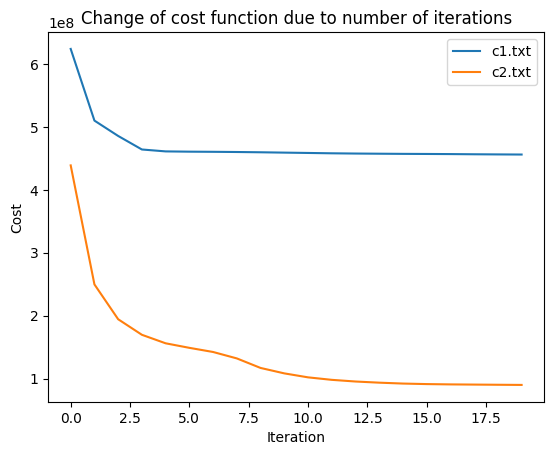
\includegraphics[width=0.8\textwidth]{q2/euclidean.png}
    \caption{Change of cost function due to the number of iteration.}
    \label{fig:euclidean_vs_iterations}
\end{figure}

The percentage change in cost after $10$ iterations of the $k$-Means
algorithm when the cluster centroids are initialized using \path{c1.txt} is $26.48\%$ 
compared to $76.7\%$ when using \path{c2.txt}. This indicates that the clustering achieved 
with \path{c1.txt} as initial centroids is more stable and closer to convergence after $10$ 
iterations of the $k$-means algorithm. Centroids in \path{c1.txt} are chosen randomly, which 
provides a more diverse starting point, allowing the algorithm to explore different regions 
of the data space. On the other hand, \path{c2.txt} initializes centroids that are as far apart 
as possible, but this may not always lead to the best clustering, especially if the data 
does not naturally separate into distinct clusters.

% Question 2(b)
\newquestion{2(b)}

\begin{figure}[htbp]
    \centering
    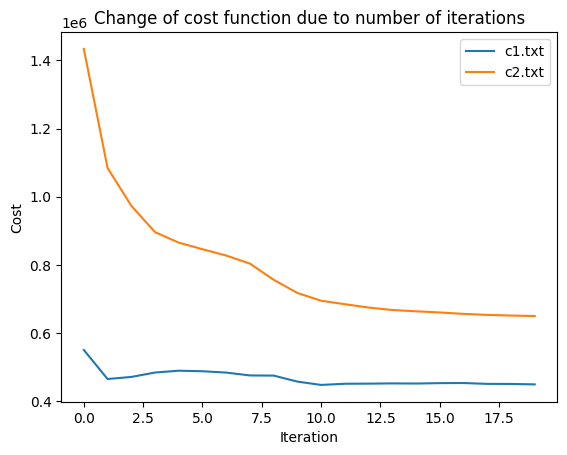
\includegraphics[width=0.8\textwidth]{q2/manhattan.png}
    \caption{Change of cost function due to the number of iteration.}
    \label{fig:euclidean_vs_iterations}
\end{figure}

In this case, the initialization method using \path{c1.txt} as initial centroids resulted in 
a lower percentage change in cost ($18.65\%$) compared to using \path{c2.txt} as initial 
centroids ($51.55\%$). Therefore, the option of initial centroids selected using \path{c1} is better.
Explanation for why this might be is stated in 2(a).

% Question 3(a)
\newquestion{3(a)}

Derivation of $E$:
\begin{align*}
    \epsilon_{iu} &= \frac{\delta}{\delta R_{ij}} E \\
    &= \frac{\delta}{\delta R_{ij}} \left( \left( \sum_{(i,u) \in ratings} (R_{iu} - q_i \cdot p_u^T)^2 \right) + \lambda \left[ \sum_u \left\lVert p_u \right\rVert^2 + \sum_i \left\lVert q_i \right\rVert^2 \right] \right) \\
    &= 2 \left( R_{iu} - q_i \cdot p_u^T \right) \text{.}
\end{align*}
Last equality holds, because there is only one $R_{iu}$ for specific $i$ and $u$ in the expression $E$. We can find it in the first sum.

Using Stochastic Gradient Descent, we update matrices $P$ and $Q$ as follows:
\begin{align*}
    P &\leftarrow P - \eta \nabla E \\
    Q &\leftarrow Q - \eta \nabla E \text{.}
\end{align*}

Here each column of matrices $p_u$ and $q_i$ are updated to
\begin{align*}
    p_u &\leftarrow p_u + \eta (\epsilon_{iu} q_i - 2 \lambda p_u) \\
    q_i &\leftarrow q_i + \eta (\epsilon_{iu} p_u - 2 \lambda q_i) \text{.}
\end{align*}


% Question 3(b)
\newquestion{3(b)}

I chose $\eta = 8 \cdot 10^{-4}$, by which I got the following graph:
\begin{figure}[htbp]
    \centering
    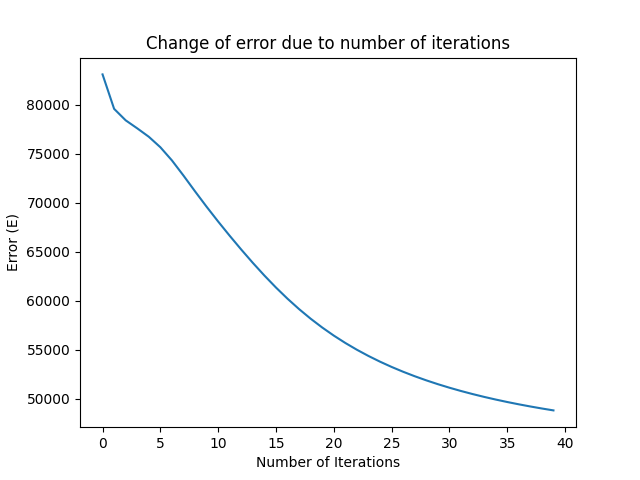
\includegraphics[width=0.8\textwidth]{q3/error.png}
    \caption{Change of error due to the number of iteration.}
    \label{fig:error_vs_iterations}
\end{figure}

% Question 4(a)
\newquestion{4(a)}

Each row $i$ in the matrix $R$ represents the items that user $i$ likes. The element in the $i$-th row and $i$-th column of the product matrix $T = R \cdot R^T$, denoted as $T_{ii}$, represents the number of items that user $i$ likes. Similarly, the element in the $i$-th row and $j$-th column of the product matrix $T$, denoted as $T_{ij}$, represents the number of items that both users $i$ and $j$ like.

To elaborate further, the $i$-th element on the diagonal $T_{ii}$ is the sum of the squares of elements in the $i$-th row of matrix $R$. Since all elements of $R$ are either $1$ or $0$, $T_{ii}$ exactly equals the sum of elements in row $i$ of matrix $R$. As each row represents items that user $i$ liked, this sum corresponds to the number of items liked by user $i$.

The elements in the $i$-th row and $j$-th column of matrix $T$ are obtained through the dot product of row $i$ and row $j$ of matrix $R$. In the dot product, we sum up the multiplications of corresponding elements of the two vectors. A factor in this sum is nonzero only if both corresponding elements in the vectors are nonzero. Since each row represents items that user $i$ liked, a nonzero factor implies that both users $i$ and $j$ liked the same item. The sum of such products precisely represents the number of elements that both users $i$ and $j$ like.

An example provided in the homework instructions clarifies this concept: let $R$ be the matrix in which a $1$ in the $i$-th row and $j$-th column indicates that user $i$ likes item $j$, while a $0$ indicates that they do not like it.

\[
R =
\begin{bmatrix}
    1 & 0 & 1 \\
    1 & 0 & 0 \\
    1 & 1 & 1 \\
    0 & 0 & 1
\end{bmatrix}
\]

Compute the product matrix 
\[
T = R \cdot R^T = 
\begin{bmatrix}
    1 & 0 & 1 \\
    1 & 0 & 0 \\
    1 & 1 & 1 \\
    0 & 0 & 1
\end{bmatrix}
\begin{bmatrix}
    1 & 1 & 1 & 0 \\
    0 & 0 & 1 & 0 \\
    1 & 0 & 1 & 1 \\
\end{bmatrix}
= 
\begin{bmatrix}
    2 & 1 & 2 & 1 \\
    1 & 1 & 1 & 0 \\
    2 & 1 & 3 & 1 \\ 
    1 & 0 & 1 & 1 \\
\end{bmatrix}
\]

Let's observe the third element on the diagonal, $T_{22}$. Its value is $1$. From matrix $R$, we can see that user $2$ likes only the first item, hence only one item.

Let's also look at element $T_{13}$. Its value is $2$. From matrix $R$, we observe that users $1$ and $3$ both like the first and third items, while the second item is liked only by the third user. Hence, the number of items that both the first and third users like is $2$.

% Question 4(b)
\newquestion{4(b)}

Matrix $Q^{-1/2}$ provides normalization of column vectors. If $r_i = (r_{1i} \dots r_{mi})^T$, 
$i = 1 \dots n$, represents the $i$-th column of matrix $R$, then the sum of squares of non-zero elements 
in this column, $q_i = \sum_{k=1}^{m} r_{ki}^2$, is exactly the $i$-th element on the diagonal of 
$Q$. The equation $$\frac{1}{\sqrt{q_i}} = \frac{1}{\sqrt{\sum_{k=1}^{m} r_{ki}^2}} = \frac{1}{\left\lVert r_i \right\rVert }$$
represents the $i$-th element on the diagonal of $Q^{-1/2}$.

Therefore $RQ^{-1/2}$ can be rewriten as 
$$ RQ^{-1/2} = 
\begin{bmatrix}
    r_{1} & \cdots & r_{n}
\end{bmatrix}
\begin{bmatrix}
    \frac{1}{\left\lVert r_1 \right\rVert } && \\
    & \ddots & \\
    && \frac{1}{\left\lVert r_n \right\rVert }
\end{bmatrix}
= 
\begin{bmatrix}
    \frac{r_{1}}{\left\lVert r_1 \right\rVert} & \cdots & \frac{r_{n}}{\left\lVert r_n \right\rVert}
\end{bmatrix} \text{,}
$$
where we denote the $i$-th column of $R$ as $r_i$.


% Similarly we show that 
% $$ Q^{-1/2}R^T = 
% \begin{bmatrix}
%     \frac{1}{\left\lVert r_1 \right\rVert } && \\
%     & \ddots & \\
%     && \frac{1}{\left\lVert r_n \right\rVert }
% \end{bmatrix}
% \begin{bmatrix}
%     r_{1}^T \\
%     \vdots \\
%     r_{n}^T  
% \end{bmatrix}
% = 
% \begin{bmatrix}
%     \frac{r_{1}^T}{\left\lVert r_1 \right\rVert} \\
%     \vdots \\
%     \frac{r_{n}^T}{\left\lVert r_n \right\rVert} 
% \end{bmatrix}
% $$

In part a), we proved that each element of a product of a matrix $A$ and its transpose $A^T$, $AA^T$, 
is a dot product of row vectors. Similarly, we can show that each element of $A^TA$ is a dot product of column vectors.

Notice that the transpose of matrix $RQ^{-1/2}$ is $Q^{-1/2}R$ by calculation:
$$(RQ^{-1/2})^T = (Q^{-1/2})^T R^T = Q^{-1/2} R^T \text{,}$$
where in the second equality we used the fact that the transpose of a diagonal matrix is the matrix itself.

Therefore, each element of $Q^{-1/2} R^T RQ^{-1/2}$ is a dot product of column vectors of $RQ^{-1/2}$. A dot product of the $i$-th and $j$-th columns of $RQ^{-1/2}$ is $\frac{r_i \cdot r_j}{\left\lVert r_i \right\rVert \cdot \left\lVert r_j \right\rVert}$.

Combining all the elements, we obtain $$\left[ \frac{r_i \cdot r_j}{\left\lVert r_i \right\rVert  \left\lVert r_j \right\rVert} \right]_{ij=1}^{n} \text{.}$$ 
This is precisely matrix $S_I$, as every element represents the cosine similarity of item $i$ and item $j$.


Now, we would like to derive an expression for $S_U$. Let's denote $r_i = (r_{i1} \dots r_{in})$, 
$i = 1 \dots m$, as the $i$-th row of matrix $R$. The number of non-zero elements in row $i$, 
$p_i = \sum_{k=1}^{n} r_{ik}^2$, is exactly the $i$-th element on the diagonal of $P$. The 
equation
$$\frac{1}{\sqrt{p_i}} = \frac{1}{\sqrt{\sum_{k=1}^{n} r_{ik}^2}} = \frac{1}{\left\lVert r_i \right\rVert }$$
represents the $i$-th element on the diagonal of $P^{-1/2}$. Calculating,
$$ P^{-1/2}R = 
\begin{bmatrix}
    \frac{1}{\left\lVert r_1 \right\rVert } && \\
    & \ddots & \\
    && \frac{1}{\left\lVert r_n \right\rVert }
\end{bmatrix}
\begin{bmatrix}
    r_{1} \\
    \vdots \\ 
    r_{m}
\end{bmatrix}
= 
\begin{bmatrix}
    \frac{r_{1}}{\left\lVert r_1 \right\rVert} \\ 
    \vdots \\ 
    \frac{r_{n}}{\left\lVert r_n \right\rVert}
\end{bmatrix} \text{.}
$$

.

From part a), we know that each element of a product of a matrix $A$ and its transpose $A^T$, $AA^T$, is a dot product 
of row vectors. Therefore, if we write $S_U = (P^{-1/2}R) (P^{-1/2}R)^T = P^{-1/2} R R^T P^{-1/2}$, we can express $S_U$ as
$$\left[ \frac{r_i \cdot r_j}{\left\lVert r_i \right\rVert  \left\lVert r_j \right\rVert} \right]_{ij=1}^{m} \text{.}$$

% Question 4(c)
\newquestion{4(c)}

For user-user collaborative filtering denote users with $u_1 \dots u_m$ and write cosine similarity of user $u$ to other users in a 
vector $$S_u = \left( \text{cos-sim}(u_1, u) \dots \text{cos-sim}(u_m, u)\right) \text{.}$$ Write a column of $R$ for item $s$ as 
$$R_s = (R_{u_1, s} \dots R_{u_m, s}) \text{.}$$ 

We see that expression $r_{u,s}$ is just a dot product of those two vectors:
$$r_{u,s} = \sum_{x \in users} \text{cos-sim} (x, u) \cdot R_{x,s} = 
\begin{bmatrix}
    \text{cos-sim}(u_1, u) & \cdots & \text{cos-sim}(u_m, u)
\end{bmatrix}
\begin{bmatrix}
    R_{u_1, s} \\
    \vdots \\
    R_{u_m, s}
\end{bmatrix} 
= S_u^T \cdot R_s \text{.}$$

Hence, we can calculate $r_{u,s}$ by multipling $u$-th row of matrix $S_U$, defined in part b), with $s$-th column of matrix $R$.
From part b) we know that we can write $S_U$ as $S_U = P^{-1/2} R R^T P^{-1/2}$. Therefore we can write $\Gamma = S_U \cdot R = P^{-1/2} R R^T P^{-1/2} R$.

For item-item collaborative filtering denote items with $i_1 \dots i_n$ and write cosine similarity of item $s$ to other items in a 
vector $$S_s = \left( \text{cos-sim}(i_1, s) \dots \text{cos-sim}(i_n, s)\right) \text{.}$$ Write a row of $R$ for user $u$ as
$$R_u = (R_{u, i_1} \dots R_{u, i_n}) \text{.}$$ 

We see that expression $r_{u,s}$ is just a dot product of those two vectors:
$$r_{u,s} = \sum_{x \in items} R_{u, x} \cdot \text{cos-sim} (x, s) = 
\begin{bmatrix}
    R_{u, i_1} & \dots & R_{u, i_n}
\end{bmatrix}
\begin{bmatrix}
    \text{cos-sim}(i_1, s) \\
    \vdots \\
    \text{cos-sim}(i_n, s)
\end{bmatrix}
= R_u^T \cdot S_s \text{.}$$

Hence, we can calculate $r_{u,s}$ by multipling $u$-th row of matrix $R$ with $s$-th column of matrix $S_I$, defined in part b).
From part b) we know that we can write $S_I$ as $S_I = Q^{-1/2} R^T RQ^{-1/2}$. Therefore we can write $\Gamma = R \cdot S_I = R Q^{-1/2} R^T RQ^{-1/2}$.


% Question 4(d)
\newquestion{4(d)}

TV shows with the highest recommendation scores for Alex
for the user-user collaborative filtering:
\begin{itemize}
    \item Two and a Half Men
    \item NBC 4 at Eleven
    \item 2009 NCAA Basketball Tournament
    \item Family Guy
    \item FOX 28 News at 10pm
\end{itemize}

TV shows with the highest recommendation scores for Alex
for the item-item collaborative filtering:
\begin{itemize}
    \item Access Hollywood
    \item 2009 NCAA Basketball Tournament
    \item NBC 4 at Eleven
    \item Family Guy
    \item FOX 28 News at 10pm
\end{itemize}


% Information sheet
% Fill out the information below (this should be the last page of your assignment)
\addinformationsheet
\vfill

{\Large
\textbf{Your name:} Lucija Fekonja  % Put your name here
\\
\\
\textbf{Email:} lf90992@student.uni-lj.si{\hspace*{3cm}}  % Put your e-mail here
\textbf{SUID:} 27232071  % Put your student ID here
\\*[2ex] 
}
Discussion Group: Nik Mrhar   % List your study group here
\\
\vfill\vfill
I acknowledge and accept the Honor Code.\\*[3ex]
\bigskip
\textit{(Signed)} 
L. F.  % Replace this line with your initials
\vfill






\end{document}